It is important that any image is fed into the network crop by crop. Meaning that for each crop there is separate embedding. In this section the embeddings from ine images were not combined in any way togther and were analysed separately. However, it is strongly recommended for a further research to evaluate all the experiments by finding the projections in the lower space not only of separate crops, but of the image as the whole. For example, simply by averaging the embeddings for each crops from one image. For all of the experiments a model trained on nuclei dataset was used.

UNet embedding consists is of size $16 \times 16 \times 256$ and can be flattened into a $655536$-dimensional vector. In order to comprehend the embeddings for us as humans, one has to first apply any dimensionality reduction algorithm on them. One of the options is to compress the vector to 2D or 3D-dimentional representation, which can be easily comprehendable by humans.
\begin{figure}[htb]
	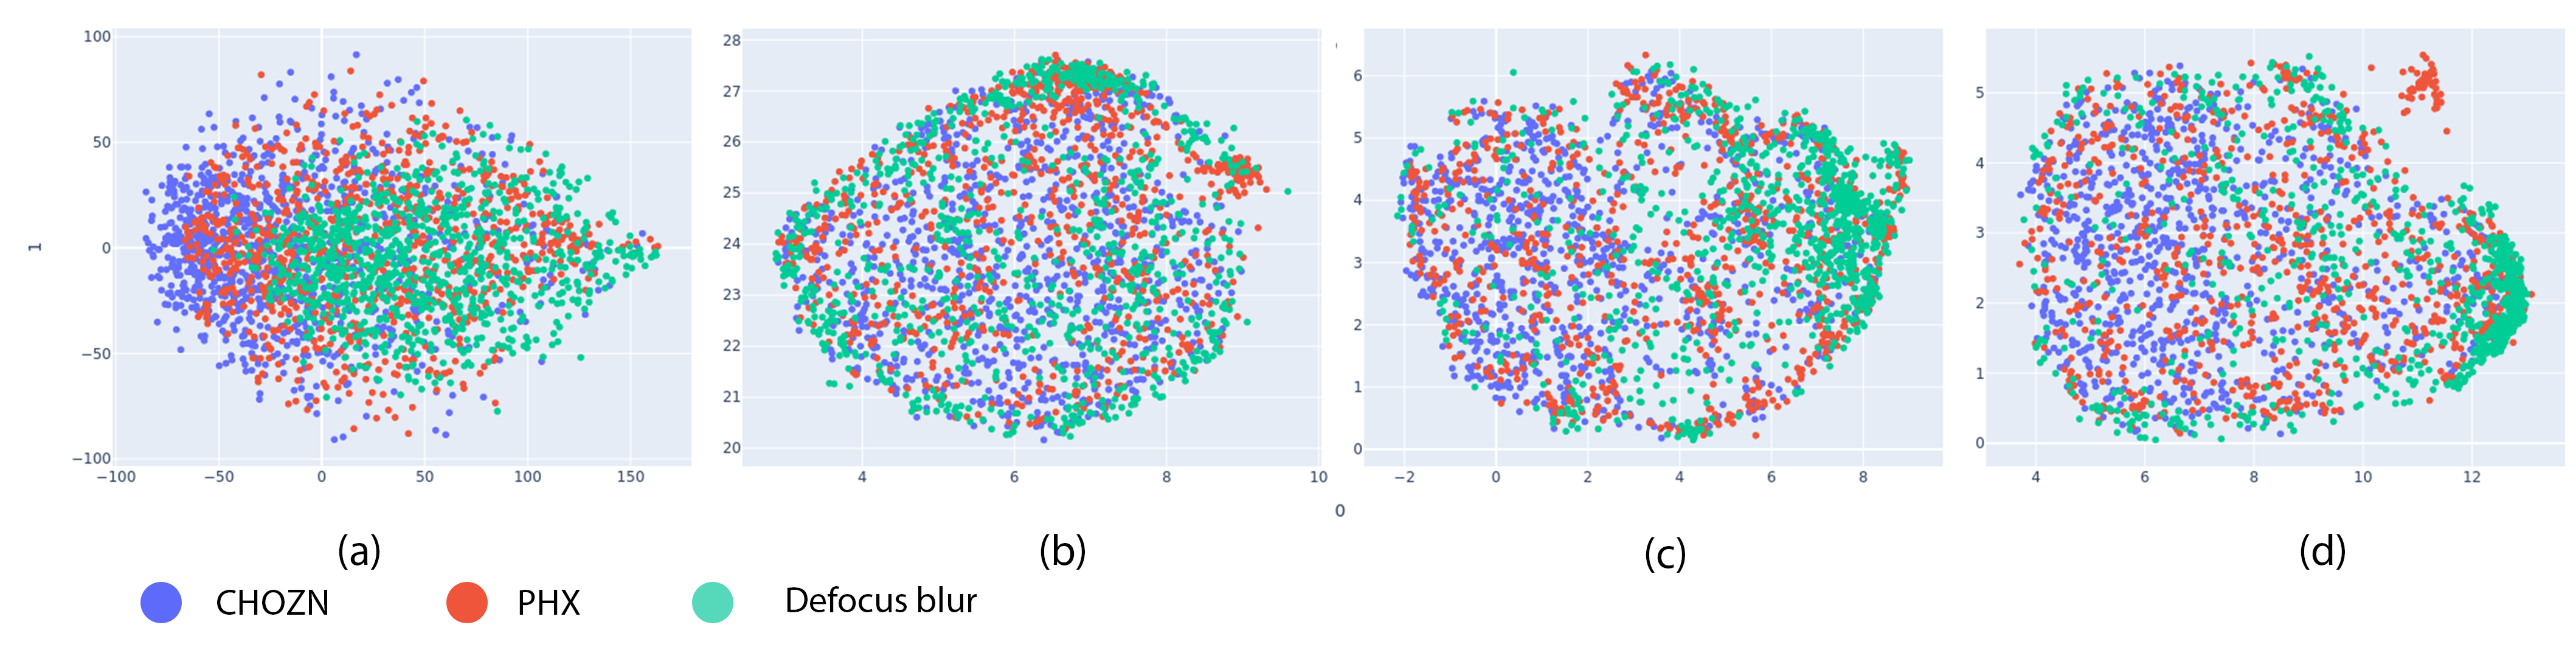
\includegraphics[width=\linewidth]{bilder/unet-embeddings/umap-pca-embeddings.png}
	\caption{(a) PCA, (b) UMAP, (c) combination of PCA and UMAP with 10 and (d) 50 components}\label{fig:umap-pca-embeddings}
\end{figure}

In this case a two-dimensional representation was chosen. With the help of PCA, UMAP and their combination the embeddings were projected into 2D space. In Figure \ref{fig:umap-pca-embeddings} one can the clouds of dots, where each dot represents a projected UNet embedding of a crop. Both research questions are addressed here: clustering based on the phenotype (CHOZN or PHX) and clustering based on the corruptions in the inputs. It is very important here that corruted data was not used in training of any of dimensionality reduction methods. The goal was to use only the data available in trianing dataset, find the transformation of high-dimentional data into a lower-dimentional space and apply it to new samples. That is also why methods like t-sne \cite(t-sne) cannot be used here, because the transformation t-sne learns cannot be applied to new samples. 

From Figure \ref{fig:umap-pca-embeddings} it is clear that there is no clustering based on the phenotype is happening. However, green corrupted dots seem to clump more in groups, distributing either on one side (a, d) or around the center (b). It is also clear that the combination of UMAP with previously applied PCA works better with the increasing amount of components in PCA: dots in (d) seem to form a better cluster than dots in (c). Yet it is still not clear from this Figure how many not corrupted dots are hidden behind the cluster of the green ones --- meaning whether non corrupted crops cluster intersects severely with a corrupted one. In order to visualize that better one can use a kernel density estimate (KDE) plot presented in Figure \ref{fig:kde}. Additionally, it is clear that vanilla UMAP is not the best approach for the extreme number of dimentions as one has in this case.

\begin{figure}[htb]
	\begin{center}
		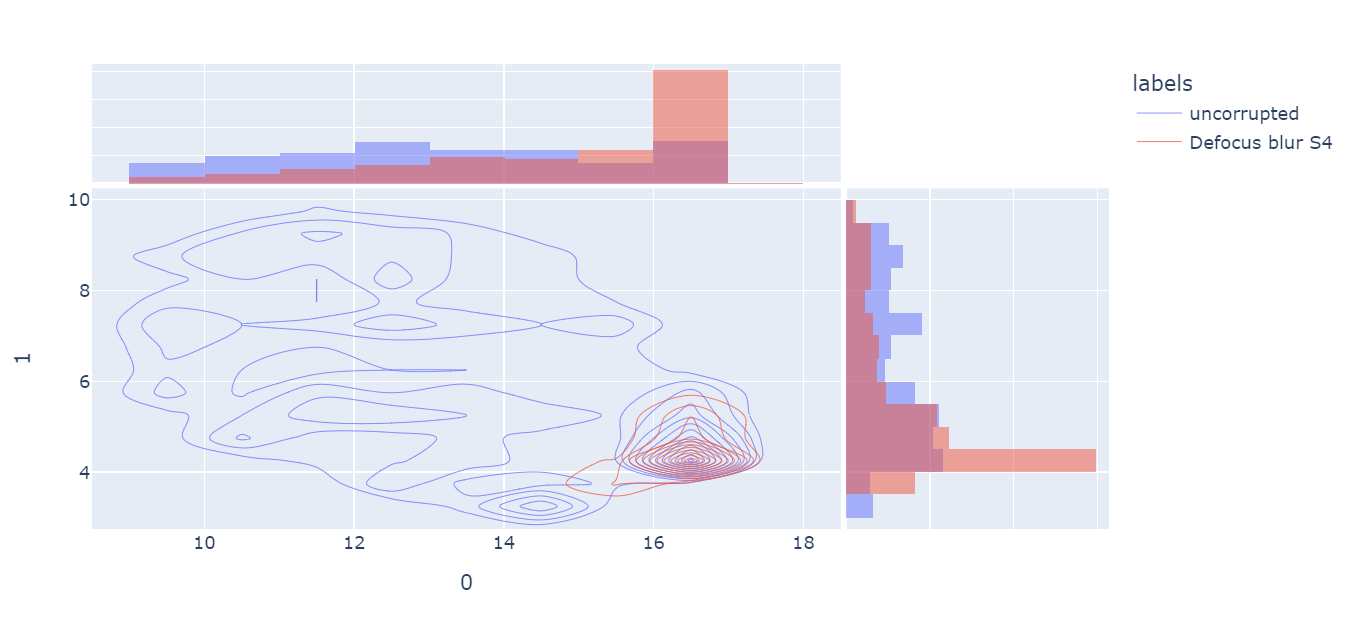
\includegraphics[width=0.6\linewidth]{bilder/unet-embeddings/kde.png}
	\caption{KDE plot of UMAP applied after PCA with 200 components}\label{fig:kde}
	\end{center}
\end{figure}

One can see that there is clearly a cluster of corrupted images here, however it also intersects with the many non corrupted crops. The quantitive evaluation of how this cluster if separable from the rest of the point is provided in section \ref{section:clustering-on-unet-embeddings}. Altough one can already state that there is a clear opportunity to differentiate between corrupted and non corrupted images, but due to clusters being not well separable the accuracy cannot be high. For further research we suggest to additionally check whether clusters may form into a high-dimensional space before projecting it into a 2D space. 
